\documentclass[border=4pt, multi, tikz]{standalone}
\usepackage{amsmath}
\usepackage{amssymb}
\usepackage{import}
\subimport{./}{init}
\usetikzlibrary{positioning}
\usetikzlibrary{calc}
\usetikzlibrary{fit}

% --- color palette ---
\colorlet{EncColor}{blue!18}
\colorlet{EncBandColor}{blue!50}
\colorlet{DecColor}{red!22!yellow!55}
\colorlet{DecBandColor}{red!55!yellow!40}
\colorlet{SlotColor}{yellow!75}
\colorlet{NCAColor}{green!35}
\colorlet{NCABandColor}{green!70}
\colorlet{EmbedColor}{green!12}
\colorlet{ReadoutColor}{red!18}
\colorlet{XAttnColor}{blue!10}

\begin{document}
\begin{tikzpicture}
\tikzstyle{connection}=[-Stealth, line width=0.5mm,
    every node/.style={sloped,allow upside down}, draw=\edgecolor, opacity=0.85]
\tikzstyle{condarrow}=[-Stealth, line width=0.5mm, dashed,
    draw={rgb:blue,5;magenta,2;black,2}, opacity=0.9]

% Vertical-bar layer block for transformer sub-layers stacked L->R
\tikzstyle{tflayer}=[draw, rounded corners=1.2pt, line width=0.3pt,
    minimum width=0.32cm, minimum height=1.35cm, inner sep=1pt]

% =====================================================================
% TOP ROW : symbolic autoencoder (NON-spatial activations, flat 2D)
% =====================================================================
\def\YTop{6.5}

% --- input game spec ---
\node[draw, rounded corners=2pt, fill={gray!8},
      font=\tiny\ttfamily, align=left, inner sep=3pt,
      text width=2.5cm, anchor=east] (spec) at (1.0,\YTop)
{title sokoban\\
=========\\
objects\\
=========\\
\textbf{Player} \textbf{Crate}\\
\textbf{Wall} \textbf{Target}\\
=========\\
rules\\
=========\\
{[}\textbf{>} Player | Crate{]}\\
~->{[}|\textbf{>}P. \textbf{>}Cr.{]}};
\node[font=\scriptsize\itshape, anchor=south] at (spec.north) {game spec};
\node[font=\tiny, anchor=north, text=black!60] at (spec.south)
    {tokens $\in\,\mathbb{Z}^{S}$};

% --- Encoder: 3 vertical bars stacked left-to-right
%     (2 self-attn + 1 K-query cross-attn -- the perceiver readout)
\node[tflayer, fill=EncColor]   (encS1) at (2.6, \YTop) {};
\node[tflayer, fill=EncColor, right=0.06cm of encS1] (encS2) {};
\node[tflayer, fill=EncBandColor, right=0.06cm of encS2] (encX)  {};
\node[font=\tiny, rotate=90, inner sep=0pt] at (encS1) {self-attn};
\node[font=\tiny, rotate=90, inner sep=0pt] at (encS2) {self-attn};
\node[font=\tiny, rotate=90, inner sep=0pt, text=white!92!black]
    at (encX) {$K$-query x-attn};
\node[draw, rounded corners=2pt, line width=0.45pt, fit=(encS1)(encX),
      inner sep=2.5pt] (enc) {};
\node[font=\scriptsize\bfseries, anchor=south] at (enc.north)
    {Encoder $\mathrm{Enc}_\phi$};
\node[font=\tiny, anchor=north, text=black!60] at (enc.south)
    {$S{\times}64$};

% --- Slots z : K=16 horizontal stripes (NOT spatial) ---
\def\SlotsX{4.85}
\node[draw, rounded corners=1.5pt, fill=SlotColor, line width=0.4pt,
      minimum width=0.85cm, minimum height=1.55cm, anchor=center]
      (slots) at (\SlotsX, \YTop) {};
\foreach \y in {-0.6,-0.45,-0.3,-0.15,0.0,0.15,0.3,0.45,0.6} {
  \draw[gray!60, line width=0.18pt]
      ($(slots.west)+(0.05, \y)$) -- ($(slots.east)+(-0.05, \y)$);
}
\node[font=\scriptsize\bfseries, anchor=south] at (slots.north) {slots $z$};
\node[font=\tiny, anchor=north, text=black!65, align=center] at (slots.south)
    {$K{=}16$ vectors,\\each $\in\,\mathbb{R}^{64}$};

% --- Decoder: 4 vertical bars stacked left-to-right ---
\node[tflayer, fill=DecColor]   (decL1) at (6.65, \YTop) {};
\node[tflayer, fill=DecColor, right=0.06cm of decL1] (decL2) {};
\node[tflayer, fill=DecColor, right=0.06cm of decL2] (decL3) {};
\node[tflayer, fill=DecBandColor, right=0.06cm of decL3] (decL4) {};
\foreach \n in {decL1, decL2, decL3, decL4}
  \node[font=\tiny, rotate=90, inner sep=0pt] at (\n) {causal\,+\,x-attn};
\node[draw, rounded corners=2pt, line width=0.45pt, fit=(decL1)(decL4),
      inner sep=2.5pt] (dec) {};
\node[font=\scriptsize\bfseries, anchor=south] at (dec.north)
    {Decoder $\mathrm{Dec}_\psi$};
\node[font=\tiny, anchor=north, text=black!60] at (dec.south)
    {$S{\times}|V|$};

% --- reconstructed spec ---
\node[draw, rounded corners=2pt, fill={gray!8},
      font=\tiny\ttfamily, align=left, inner sep=3pt,
      text width=2.5cm, anchor=west] (recon) at (10.4,\YTop)
{title sokoban\\
=========\\
objects\\
=========\\
\textbf{Obj0} \textbf{Obj1}\\
\textbf{Obj2} \textbf{Obj3}\\
=========\\
rules\\
=========\\
{[}\textbf{>} Obj0 | Obj1{]}\\
~->{[}|\textbf{>}O0 \textbf{>}O1{]}};
\node[font=\scriptsize\itshape, anchor=south] at (recon.north) {reconstructed spec};
\node[font=\tiny, anchor=north, text=black!60] at (recon.south)
    {logits over $|V|$};

% --- AE flow ---
\draw[connection] (spec.east) -- (enc.west);
\draw[connection] (enc.east)  -- (slots.west);
\draw[connection] (slots.east)-- (dec.west);
\draw[connection] (dec.east)  -- (recon.west);

% --- token CE loss label ---
\node[font=\scriptsize\itshape, text=red!55!black, anchor=south]
    at (5.5, 8.7) {$\mathcal{L}_{\text{tok}}$\,:\, token cross-entropy};

% =====================================================================
% BOTTOM ROW : dynamics (SPATIAL activations, 3D boxes)
%   Defined first so the cross-attn block can reference nca-north.
%   xlabel = channels (bottom front edge).
%   zlabel = spatial size H x W (bottom right diagonal).
% =====================================================================

% --- input state image ---
\node[draw, rounded corners=2pt, line width=0.5pt, inner sep=2pt, anchor=east]
    (sin) at (0.7, 0) {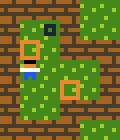
\includegraphics[width=1.7cm]{state_in.png}};
\node[font=\scriptsize\itshape, anchor=north] at (sin.south) {$s_t$};
\node[font=\tiny, anchor=south, text=black!60] at (sin.north)
    {$C{\times}H{\times}W$};

% --- action chip ---
\node[draw, rounded corners=2pt, fill=yellow!25,
      font=\scriptsize, inner sep=2pt] (act) at (1.5, 0)
    {$a_t {=} \texttt{down}$};

% --- embed: 1x1 dense, output is hidden grid h^(0) with 128 channels ---
% (xlabel = channels on bottom front; zlabel = spatial size H x W)
\pic[shift={(2.6,0,0)}] at (0,0,0)
    {Box={
        name=embed,
        caption=embed,
        xlabel={{128,}},
        zlabel={},
        fill=EmbedColor,
        height=14,
        width=2,
        depth=14
        }
    };

% --- NCA stack: bands = T=20 shared-weight steps; each band has 128 chans ---
\pic[shift={(4.4,0,0)}] at (0,0,0)
    {RightBandedBox={
        name=nca,
        caption={NCA body ($T{=}20$ steps, shared)},
        xlabel={{128,,,,,,,,}},
        zlabel={$H{\times}W$},
        fill=NCAColor,
        bandfill=NCABandColor,
        height=16,
        width={1.4,1.4,1.4,1.4,1.4,1.4,1.4,1.4},
        depth=16
        }
    };

% --- readout: 1x1 dense, output is C-channel logits at H x W ---
% (xlabel must be numeric for pgf; we add the C label as a TikZ node)
\pic[shift={(8.4,0,0)}] at (0,0,0)
    {Box={
        name=readout,
        caption=readout,
        xlabel={{,}},
        zlabel={},
        fill=ReadoutColor,
        height=14,
        width=2,
        depth=14
        }
    };
\node[font=\small, anchor=north] at ($(readout-south)+(0,-0.1)$) {$C$};

% --- output state image ---
\node[draw, rounded corners=2pt, line width=0.5pt, inner sep=2pt, anchor=west]
    (sout) at (10.4, 0) {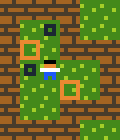
\includegraphics[width=1.7cm]{state_out.png}};
\node[font=\scriptsize\itshape, anchor=north] at (sout.south) {$\hat s_{t+1}$};

\draw[connection] (sin.east)    -- (embed-west);
\draw[connection] (embed-east)  -- (nca-west);
\draw[connection] (nca-east)    -- (readout-west);
\draw[connection] (readout-east)-- (sout.west);

% --- BCE loss label ---
\node[font=\scriptsize\itshape, text=red!55!black, anchor=north]
    at (5.5, -3.4) {$\mathcal{L}_{\text{state}}$\,:\, per-cell BCE\,+\,win BCE};

% =====================================================================
% MIDDLE : explicit cross-attention mechanism between slots and NCA.
%   Slots provide K, V (down arrow). Each NCA cell provides Q (loop).
%   Output is a per-cell context vector added into the NCA update at
%   every step.
% =====================================================================
\node[draw, rounded corners=2pt, fill=XAttnColor, line width=0.4pt,
      minimum width=2.9cm, minimum height=1.0cm, anchor=center,
      align=center, font=\scriptsize] (xattn) at (\SlotsX, 3.6)
    {rule cross-attention \textit{(every step)}\\[-1pt]
     {\tiny $\mathrm{softmax}\!\bigl(QK^{\!\top}\!/\!\sqrt{d}\bigr)\,V$}};

% Slots --> xattn :: K,V from slots
\draw[condarrow] (slots.south)
    -- node[right=0.4mm, pos=0.55, font=\tiny, text=blue!55!black]
       {keys, values} (xattn.north);

% xattn --> NCA :: per-cell context output
\draw[condarrow] (xattn.south)
    -- node[right=0.4mm, pos=0.55, font=\tiny, text=blue!55!black]
       {context} ($(nca-north)+(0,0.05)$);

% Loop: queries come from each NCA cell h^{(k)}, returned to xattn.east
\draw[->, dashed, line width=0.4mm,
      draw={rgb:blue,3;magenta,2;black,3}, opacity=0.9,
      rounded corners=4pt]
    ($(nca-north)+(0.45,0.05)$) -- ++(0,0.55) -- ++(1.6,0) -- (xattn.east);
\node[font=\tiny, text=blue!55!black, anchor=west, align=left]
    at ($(xattn.east)+(0.05,0.42)$) {$Q$ from\\each cell};


\end{tikzpicture}
\end{document}
